%
% auth: Mattijs Korpershoek
% mail: <mattijs.korpershoek@gmail.com>
%

\section{Context}

\subsection{Celad}
\begin{FrameWithSubSection}
    \begin{minipage}{0.49\textwidth}
        \begin{itemize}
            \item Some metrics
            \item Some metrics
            \item Some metrics
        \end{itemize}
    \end{minipage}
    \begin{minipage}{0.49\textwidth}
        \flushright
        
\includegraphics[height=2cm]{../../report/src/img/logocelad.jpg}
    \end{minipage}
\end{FrameWithSubSection}

\subsection{Intel}
\begin{FrameWithSubSection}
    \begin{minipage}{0.49\textwidth}
        \begin{itemize}
            \item Some metrics
            \item Some metrics
            \item Some metrics
        \end{itemize}
    \end{minipage}
    \begin{minipage}{0.49\textwidth}
        \flushright
        
\includegraphics[height=2cm]{../../report/src/img/logointel.jpg}
    \end{minipage}
\end{FrameWithSubSection}

\subsection{Android}
\begin{FrameWithSubSection}
    \begin{minipage}{0.49\textwidth}
        \begin{itemize}
            \item Some metrics
            \item Some metrics
            \item Google I/O trends left
        \end{itemize}
    \end{minipage}
    \begin{minipage}{0.49\textwidth}
        \flushright
        TODO TODO TODO android image
        
\includegraphics[height=2cm]{../../report/src/img/logocelad.jpg}
    \end{minipage}
\end{FrameWithSubSection}
\begin{FrameWithSubSection}
    \frametitle{Android architecture}
    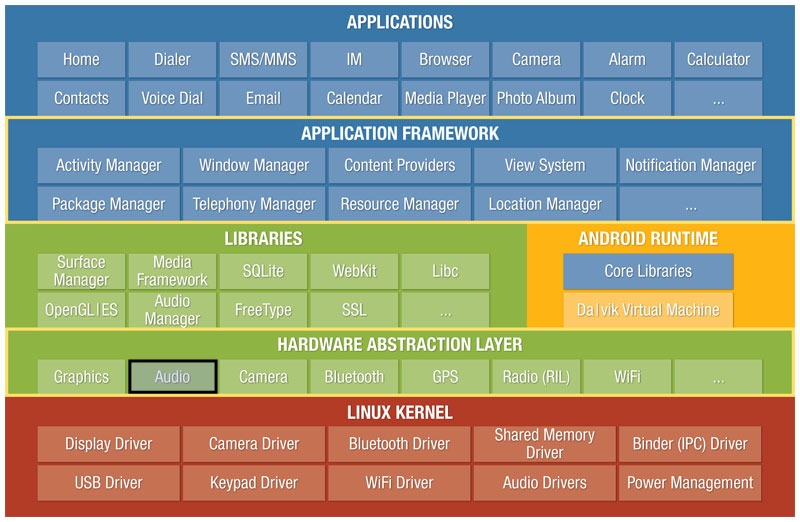
\includegraphics[width=\textwidth]{../../report/src/img/android-archi-audio-hal.jpeg}
\end{FrameWithSubSection}

\subsection{Intel Audio HAL}
\begin{FrameWithSubSection}
    \begin{block}{Hardware Abstraction Layer}
        \begin{itemize}
            \item Scalability
            \item Configurability
        \end{itemize}
    \end{block}
\end{FrameWithSubSection}

\begin{FrameWithSubSection}
    % report must be compiled before this works
    % TODO uncomment this
    % \includegraphics[width=\textwidth]{../../report/src/img/hal-architecture.pdf}
\end{FrameWithSubSection}


\subsection{Parameter-framework}
\begin{FrameWithSubSection}
    \begin{minipage}{0.49\textwidth}
    \begin{block}{Structure description}
        \begin{itemize}
            \item Structured in a tree
            \item XML description
        \end{itemize}
    \end{block}
    \end{minipage}
    \begin{minipage}{0.49\textwidth}
    %\fbox{\begin{minipage}{6cm}
    %        \dirtree{%
    %            .1 audio.
    %                .2 microphone.
    %                    .3 echo\_cancellation.
    %                        .4 enable.
    %                        .4 configuration.
    %                            .5 gain.
    %                            .5 coefficient.
    %                .2 speaker.
    %                    .3 equalizer.
    %                        .4 enable.
    %                        .4 configuration.
    %                            .5 filter.
    %                            .5 coefficient.
    %        }
    %\end{minipage}}
    \end{minipage}
\end{FrameWithSubSection}

\begin{FrameWithSubSection}
    \begin{minipage}{0.49\textwidth}
    \begin{block}{Domains description}
        \begin{itemize}
            \item Structured in a tree
            \item XML description
        \end{itemize}
    \end{block}
    \end{minipage}
    \begin{minipage}{0.49\textwidth}
        %\begin{lstlisting}[language=pfwLang]
        %    Domain:
        %        Conf: SpeakerWithEchoCancel
        %            InputDevice Is Microphone
        %            Component: audio/speaker/
        %                echo_cancellation/enable = true
        %                configuration/gain = 2
        %                configuration/coefficient = 3
        %            # -- snippet --
        %\end{lstlisting}
    \end{minipage}
\end{FrameWithSubSection}
